% !TEX program = lualatex
% Generated by new_homework.sh — Math 113 Homework 2
\documentclass[11pt]{article}

\usepackage{fontspec}
\usepackage{microtype}
\usepackage{mathtools,amssymb,amsfonts,amsthm,bm}
\usepackage{enumitem}
\usepackage{booktabs,array,xcolor}
\usepackage{geometry,fancyhdr,setspace}
\usepackage{pdfpages}
\usepackage[hidelinks]{hyperref}
\usepackage[nameinlink,noabbrev]{cleveref}

% ---------- Page and paragraph rhythm (matches lecture/solutions templates) ----------
\geometry{margin=1in,headheight=15pt}
\setstretch{1.12}
\setlength{\parindent}{0pt}
\setlength{\parskip}{0.55em plus 0.12em minus 0.08em}
\setlength{\abovedisplayskip}{0.8em plus 0.2em minus 0.1em}
\setlength{\belowdisplayskip}{0.8em plus 0.2em minus 0.1em}
\allowdisplaybreaks[3]
\setlist{leftmargin=*,topsep=0.35em,itemsep=0.15em,parsep=0pt}

% ---------- Metadata ----------
\newcommand{\studentname}{Keshav Ramamurthy}
\newcommand{\coursename}{Math 113}
\newcommand{\courselongname}{Abstract Algebra}
\newcommand{\assignment}{Homework 2}
\newcommand{\term}{Fall 2026}

% ---------- Core notation (same as ~/.config/nvim/textemplate.tex) ----------
\newcommand{\N}{\mathbb{N}}
\newcommand{\Z}{\mathbb{Z}}
\newcommand{\Q}{\mathbb{Q}}
\newcommand{\R}{\mathbb{R}}
\newcommand{\C}{\mathbb{C}}
\newcommand{\F}{\mathbb{F}}
\newcommand{\K}{\mathbb{K}}
\newcommand{\E}{\mathbb{E}}
\newcommand{\Prob}{\mathbb{P}}
\newcommand{\1}{\mathbf{1}}
\newcommand{\eps}{\varepsilon}
\newcommand{\dd}{\,\mathrm{d}}
\newcommand{\abs}[1]{\left\lvert#1\right\rvert}
\newcommand{\norm}[1]{\left\lVert#1\right\rVert}
\newcommand{\ip}[2]{\left\langle#1,#2\right\rangle}
\newcommand{\set}[1]{\left\{#1\right\}}
\newcommand{\ceil}[1]{\left\lceil#1\right\rceil}
\newcommand{\floor}[1]{\left\lfloor#1\right\rfloor}
\newcommand{\given}{\,\middle\vert\,}
\newcommand{\indep}{\perp\!\!\!\perp}
\newcommand{\wh}[1]{\widehat{#1}}
\newcommand{\deriv}[2]{\frac{\mathrm{d}#1}{\mathrm{d}#2}}
\newcommand{\pderiv}[2]{\frac{\partial#1}{\partial#2}}
\newcommand{\lto}{\longrightarrow}
\newcommand{\st}{\text{ such that }}
\DeclareMathOperator{\Aut}{Aut}
\DeclareMathOperator{\End}{End}
\DeclareMathOperator{\Gal}{Gal}
\DeclareMathOperator{\Hom}{Hom}
\DeclareMathOperator{\Ker}{ker}
\DeclareMathOperator{\im}{im}
\DeclareMathOperator{\rank}{rank}
\DeclareMathOperator{\nullity}{nullity}
\DeclareMathOperator{\Span}{span}
\DeclareMathOperator{\tr}{tr}
\DeclareMathOperator{\diag}{diag}
\DeclareMathOperator{\spec}{spec}
\DeclareMathOperator{\ord}{ord}
\DeclareMathOperator{\supp}{supp}
\DeclareMathOperator{\diam}{diam}
\DeclareMathOperator{\Var}{Var}
\DeclareMathOperator{\Cov}{Cov}
\DeclareMathOperator*{\argmin}{arg\,min}
\DeclareMathOperator*{\argmax}{arg\,max}

% ---------- Statement environments ----------
\newtheorem{problem}{Problem}
\newtheorem{theorem}{Theorem}
\newtheorem{lemma}{Lemma}
\newtheorem{proposition}{Proposition}
\newtheorem{corollary}{Corollary}
\theoremstyle{definition}
\newtheorem{definition}{Definition}
\newtheorem{example}{Example}
\newtheorem{remark}{Remark}

% ---------- Solution machinery (matches solutions.tex / textemplate.tex) ----------
\newenvironment{solution}{\begin{proof}[Solution]}{\end{proof}}
\newenvironment{answer}{\begin{proof}[Answer]}{\end{proof}}
\renewcommand{\qedsymbol}{$\square$}
\newcommand{\exercise}[1]{%
  \par\goodbreak\medskip\noindent\textbf{Exercise #1}\par\nopagebreak\smallskip\nopagebreak}
\newcommand{\exref}[1]{\textsf{\textbf{Exercise~#1}}}
\newenvironment{claim}{\par\smallskip\noindent\textbf{Claim.}\ }{\par\smallskip}
\newenvironment{idea}{\par\smallskip\noindent\textit{Idea.}\ }{\par\smallskip}
\newenvironment{proofsketch}{\par\smallskip\noindent\textbf{Proof sketch.}\ }{\par\smallskip}

% ---------- Header ----------
\pagestyle{fancy}
\fancyhf{}
\fancyhead[L]{\coursename}
\fancyhead[C]{\assignment\ — my solutions}
\fancyhead[R]{\studentname}
\fancyfoot[C]{\thepage}

\begin{document}

% ---------- Title ----------
\begin{center}
  {\Large\sffamily\bfseries \coursename\ -- \courselongname}\par\vspace{3pt}
  {\sffamily \assignment\ — my solutions}\par\vspace{3pt}
  {\small\sffamily \term\quad\textbullet\quad \studentname}
\end{center}
\medskip
\hrule
\bigskip

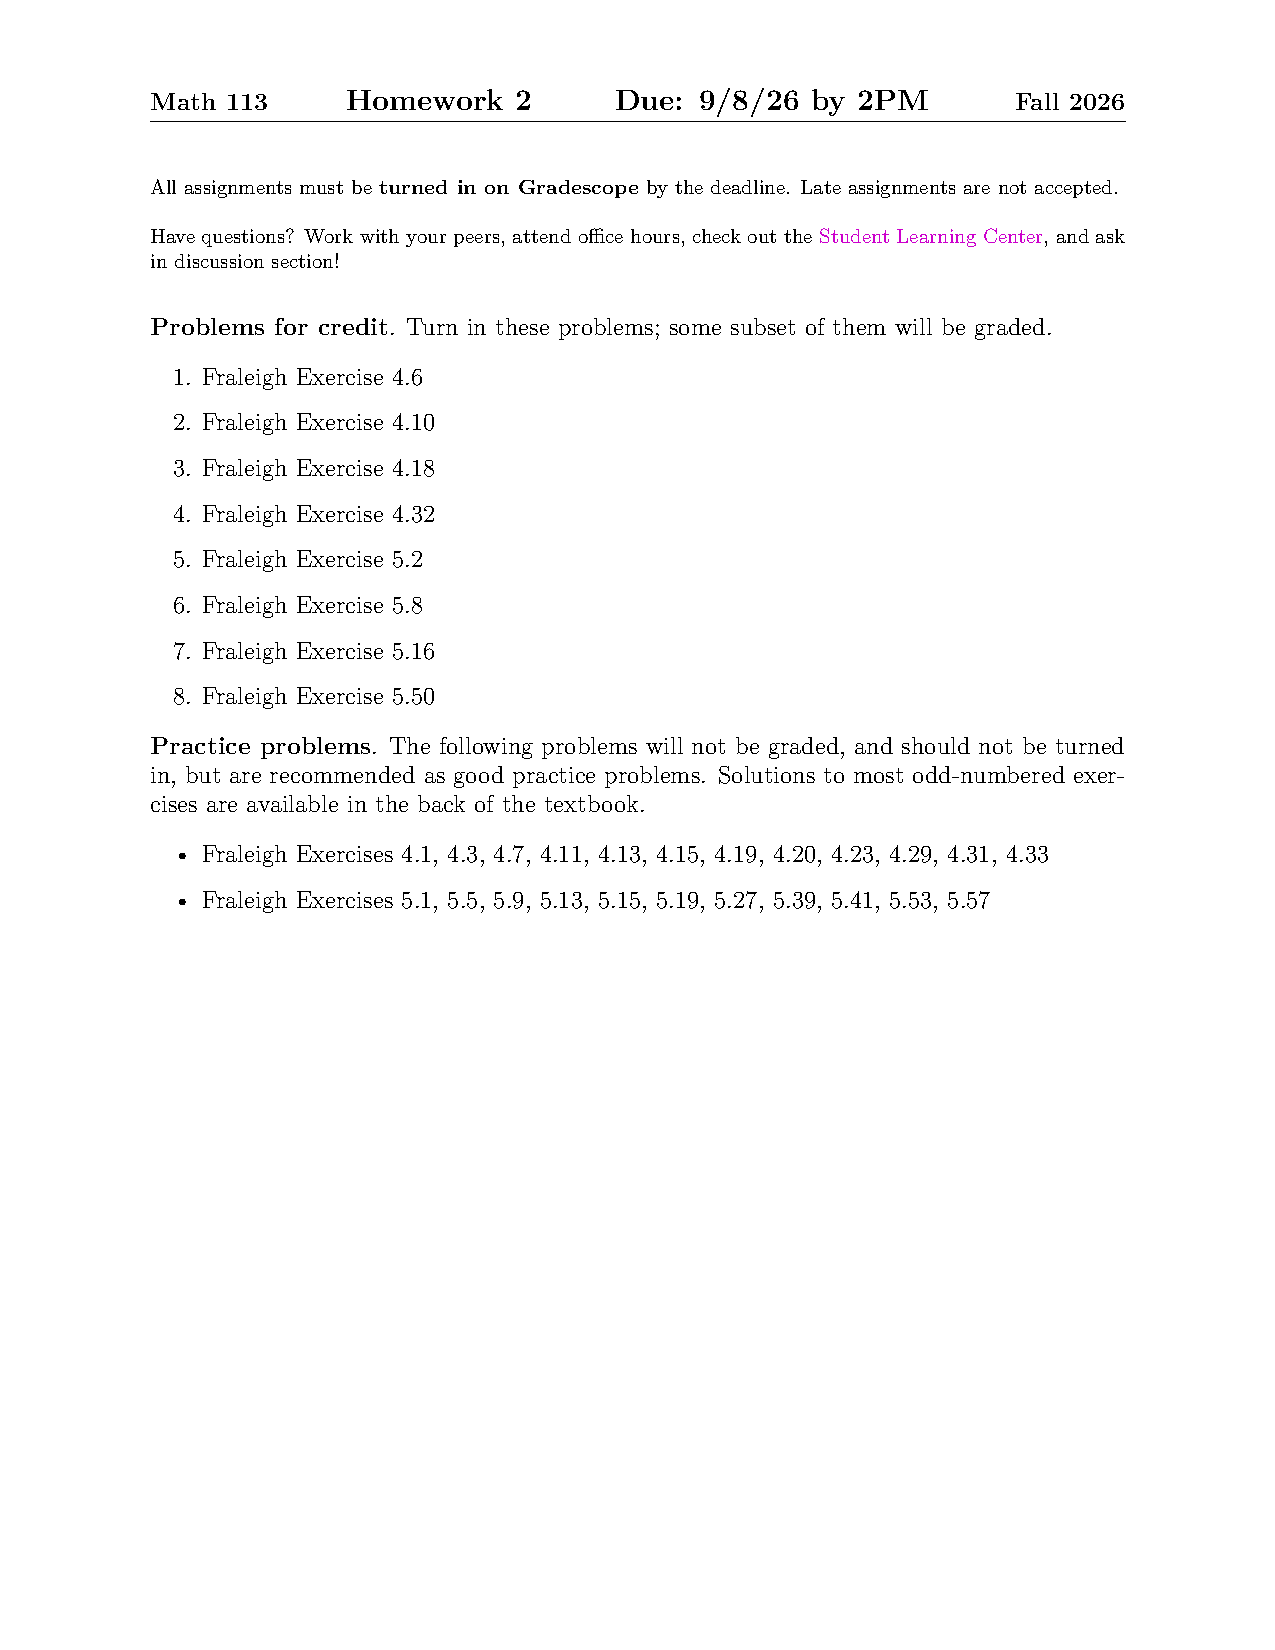
\includepdf[pages=-,pagecommand={\thispagestyle{empty}}]{hw2.pdf}
\clearpage

\section*{Solutions}
\subsubsection*{Problem 1 (Fraleigh Exercise 4.6)}
\begin{solution}
    \textbf{a) }The three necessarily axioms are associativity, existence of an inverse, and an identity
element (and closure under the operator).
\par We try this given the operator $*$ defined on $\mathbb{C}$ such that $a * b =
|ab|$
\par We have $$a * (b * c) = a * (|bc|) = |a|bc||  = |abc|$$
and 
$$(a * b) * c = (|ab|) * c = ||ab|c| = |abc|$$
so associativity holds.
\par We then see if there exists an element $e * a = a$ for all $a \in \mathbb{C}$
and we see that $\forall k \in \mathbb{C}, |k| \in \mathbb{R}.$ 
\par Thus, we can easily formulate a counterexample with a nonzero complex part, such as $1 +
i$, and we see that solving $|e \cdot (1 + i)| = 1 + i$ which has no solutions for $e
\in \mathbb{C}.$
% Write your proof, calculation, or argument here.
\end{solution}
\subsubsection*{Problem 2 (Fraleigh Exercise 4.10)}
\begin{solution}
We first check that addition is closed under $n\mathbb{Z}.$\par For $a, b \in n\mathbb{Z}$,

\par We have $\exists a', b' \in \mathbb{Z} \text{ such that } a' n = a, b' n = b.$ by
definition of $n\mathbb{Z}.$
Then, for $a, b \in n\mathbb{Z}$, so $$a + b = na' + nb' = n(a' + b') \text{ and since } a' + b' \in
\mathbb{Z} \implies n(a' + b') \in n\mathbb{Z}$$ 
0 is the identity element because $\forall k \in n\mathbb{Z}, 0 + k = k$
\par Associativity also pretty easily holds because of associativity on $(\mathbb{Z},
+)$, as 
$$a, b, c \in \mathbb{Z} \implies na, nb, nc \in n\mathbb{Z} \text{ and } na + (nb + nc) = (na + nb) + nc = na +  nb + nc$$
Notice also the existence of an additive inverse, as $$a \in \mathbb{Z} \implies -a\in
\mathbb{Z} \implies n(a), -n(a) \in n\mathbb{Z} \text{ and } -n(a) + na = 0$$
Thus, all the axioms hold, and $(n\mathbb{Z}, +)$ is a group.

\textbf{b) } We subsequently will show that $(n\mathbb{Z}, +) \simeq (\mathbb{Z}, +).$
To do so, we have to prove injectivity, surjectivity, and homomomorphism.
For the homomomorphism condition, we have to show for $(\mathbb{Z}, +)$ and
$(n\mathbb{Z}, +)$, 
$$f(x * y) = f'(x) *' f'(y)$$ or in this case: 
$$f(x + y)= f(x) + f(y) \rightarrow n(x + y) = nx + ny$$
\par \noindent\textit{Claim.} The function $f : \mathbb{Z} \rightarrow n \mathbb{Z}$ is
bijective.

\begin{proof}
    \noindent\textit{Claim.} injectivity:         For $x, y \in  \mathbb{Z} \text{ where } f(x) = f(y) \implies x = y$
    \begin{proof}
        We have since $n > 0$ that $$nx = ny \implies n(x - y) = 0 \implies x = y$$
    \end{proof}
\noindent\textit{Claim.} Surjectivity: For any $$a \in n\mathbb{Z}, \exists k \text{ such
that } nk = a$$

    \begin{proof}
        This follows directly from the definition of the set $n\mathbb{Z} = \{ni : i \in
        \mathbb{Z}\}  $
        as n must divide every element in $n\mathbb{Z}$ meaning $k = \frac{a}{n}\in \mathbb{Z} \text{ and } f(k) = a$ 
    \end{proof}
\end{proof}
Thus we are done.
% Write your proof, calculation, or argument here.
\end{solution}
\subsubsection*{Problem 3 (Fraleigh Exercise 4.18)}
\begin{solution}
    We wish to see if all $n\times n$ matrices with determinant $1$ or $-1$ under
    matrix multiplication is a group.
    \par Any matrix satisfying these conditions has an inverse as it  has a nonzero
    determinant, and this inverse for a matrix A has the condition $\det(A^{-1} ) =
    \frac{1}{\det A}$ which is either 1 or -1, closed under this condition.
    \par Along with this, matrix multiplication holds under associativity and notice the
    identity matrix \[
I_n =
\begin{pmatrix}
1 & 0 & \cdots & 0 \\
0 & 1 & \cdots & 0 \\
\vdots & \vdots & \ddots & \vdots \\
0 & 0 & \cdots & 1
\end{pmatrix}
\]
satisfies the determinant condition (has determinant 1) and for every matrix $E$ that
satisfies the conditions $I \cdot E = E$.
\par We establish closure: For matrices $A, B$ satisfying these conditions, notice
$\det(AB) = \det(A)\det(B)$ and since the product of 2 numbers in $\{-1, 1\}$ is in
$\{-1, 1\}$, so $AB$ is satisfies the original conditions (as the product of these is
also an n by n matrix)
\par Thus, we claim this is a group.
% Write your proof, calculation, or argument here..
\end{solution}
\subsubsection*{Problem 4 (Fraleigh Exercise 4.32)}
\begin{solution}
We are given that $G$ is a group, and that $\forall x \in G, x * x  = e.$ We first
consider manipulating $(a * b) * (a * b) = e$ because by closure on $G,$ $$\exists w \in
G, a * b = w \rightarrow w * w = e.$$
Manipulating that expression  yields $$(a * (b * a) * b) \rightarrow = e \rightarrow
a^{-1} * (a * (b * a) * b) * b^{-1 }= a^{-1} eb^{-1}$$
or 
$$(b * a) = a^{-1} * e *  b^{-1} = a^{-1} * b^{-1}$$
But we see that $a * a = e\implies a = a^{-1}$ due to the uniqueness of the inverse.
So we have that $(b * a) = a * b$, proving commutativity and making it an Abelian Group.
% Write your proof, calculation, or argument here.
\end{solution}
\subsubsection*{Problem 5 (Fraleigh Exercise 5.2)}
\begin{solution}
We wish to show if $\mathbb{Q}^{+}$ is a subgroup of $\mathbb{C}$ under $+.$
\par This is not true because the identity $0$ in $\mathbb{C}$ and the subsequence existence of the additive inverse in $\mathbb{C}$, the
additive inverse of $\mathbb{Q}^{+}$ does not exist, as negative numbers are not in
$\mathbb{Q}^{+}$ (and the identity $0 \not \in \mathbb{Q}^{+}$)
% $\mathbb{Q}^{+}.$ 
% Write your proof, calculation, or argument here.
\end{solution}
\subsubsection*{Problem 6 (Fraleigh Exercise 5.8)}
\begin{solution}
    $GL(n, \mathbb{R})$ is the group of $n \times n$ matrices with nonzero determinant.
\par    We wish to show if (we'll denote $H$), the set of $n \times n$ matrices with
    determinant 2 is a subgroup of $G$.
   \par  This is immediately false, because we have that for matrix $M \in H$,
    $\det M^{-1} = \frac{1}{\det M} = \frac{1}{2}$ which is not in H, so H is not closed
    under inverses. (an example being: )
    \[M =
\begin{pmatrix}
2 & 0 & \cdots & 0 \\
0 & 1 & \cdots & 0 \\
\vdots & \vdots & \ddots & \vdots \\
0 & 0 & \cdots & 1
\end{pmatrix}
\]
% Write your proof, calculation, or argument here.
\end{solution}

\subsubsection*{Problem 7 (Fraleigh Exercise 5.16)}
\begin{solution}
    \textbf{ a) }We consider the subset denoted $H$,  $H  = f \in \hat {F} \text{ such
    that } f(1) = 1.$
    \par We claim it is  $\text{not}$ a subgroup of $F$ under addition.
\par     The identity function in $F$ would be $\forall w \in \mathbb{R}, f(w) = 0.$

\par     This identity does not exist in $H$ as $\hat{F}$ describes functions that have a
    nonzero value at every point in $\mathbb{R}$, thus no  function in H can be an identity.
% Write your proof, calculation, or argument here.
\end{solution}
\subsubsection*{Problem 8 (Fraleigh Exercise 5.50)}
\begin{solution}
If the subset is closed under the binary operator $*$ of $G$, we have that $\forall a, b
\in H, a * b \in H$
We consider an arbitrary element $ a\in H.$ This will be the key to our argument, as we
will prove for an arbitrary element, it is closed under $H$, and has an identity and
inverse.
\par Notice that $H$ is finite. We can then repeatedly exponentiate $a$.
$$a, a^2, a^3, a^4, \cdots$$ and notice this must have two powers that are the same  by the pigeonhole principle.
\par We have $\exists x, y \in \mathbb{Z}^{+} \text{ such that } a^x = a^y$ and WLOG assume $x
< y$
Then, notice $a^{y - x} = e$, so $H$ has an identity.
\par We use the variable $m =y - x$.
\par If $m$ is 1, notice that $a = e$ ,and thus a is also its own inverse, 
\par If $m$ is not 1, notice that $a * a^{m - 1} =a^{m-1} * a=  a^{m} = e$, so $a^{m-1} $ is the
inverse of $a$ and recall it is closed under exponentiation.
% In order to prove it is also a subgroup, we wish 
% Write your proof, calculation, or argument here.
\end{solution}

\end{document}
